% ZHOU-SOURCE-PAGE: 131 PRINTED: 115

Using these recursive system equations and the boundary condition $Z_n=0$, we can get
$Z_1=(n-1)^2$.\footnote[4]{Even this step is not straightforward. You need to plug in the
$i$'s and try a few cases starting with $i=n-1$. The pattern will emerge and you can see
that all the terms containing $Z_{n-1},Z_{n-2},\ldots,Z_2$ cancel out.}

\subsection{Martingale and Random walk}

\noindent\emph{Random walk:} The process $\{S_n;n\geq1\}$ is called a random walk if
$\{X_i;i\geq1\}$ are IID (identical and independently distributed) random variables and
$S_n=X_1+\cdots+X_n$, where $n=1,2,\cdots$. The term comes from the fact that we can
think of $S_n$ as the position at time $n$ for a walker who makes successive random
steps $X_1,X_2,\cdots$.

If $X_i$ takes values 1 and -1 with probabilities $p$ and $1-p$ respectively, $S_n$ is
called a \emph{simple random walk} with parameter $p$. Furthermore, if $p=\frac{1}{2}$, the
process $S_n$ is a \emph{symmetric random walk}. For symmetric random walk, it's easy
to show that

\[
\E[S_n]=0\quad\text{and}\quad
\operatorname{var}(S_n)=\E[S_n^2]-\E[S_n]^2=\E[S_n^2]=n.\footnotemark[5]
\]
\footnotetext[5]{Induction again can be used for its proof. $\operatorname{var}(S_1)=\operatorname{var}(Z_1)=1$.
Induction step: If $\operatorname{var}(S_n)=n$, then we have
$\operatorname{var}(S_{n+1})=\operatorname{var}(S_n+X_{n+1})=\operatorname{var}(S_n)+\operatorname{var}(X_{n+1})=n+1$
since $X_{n+1}$ is independent of $S_n$.}

Symmetric random walk is the process that is most often tested in quantitative interviews.
The interview questions on random walk often revolve around finding the first $n$ for which
$S_n$ reaches a defined threshold $\alpha$, or the probability that $S_n$ reaches
$\alpha$ for any given value of $n$.

\noindent\emph{Martingale:} a martingale $\{Z_n,n\geq1\}$ is a stochastic process with the
properties that $\E[\lvert Z_n\rvert]<\infty$ for all $n$ and

\[
\E[Z_{n+1}\vert Z_n=z_n,Z_{n-1}=z_{n-1},\ldots,Z_1=z_1]=z_n.
\]

The property of a martingale can be extended to

\[
\E[Z_m,m>n\vert Z_n=z_n,Z_{n-1}=z_{n-1},\ldots,Z_1=z_1]=z_n,
\]

which means the conditional expected value of future $Z_m$ is the current value $Z_n$.
\footnote[6]{Do not confuse a martingale process with a Markov process. A martingale does not
need to be a Markov process; a Markov process does not need to be a martingale process,
either.}

A symmetric random walk is a martingale. From the definition of the symmetric random
walk we have

\[
S_{n+1}=\begin{cases}
S_n+1 & \text{with probability }1/2,\\
S_n-1 & \text{with probability }1/2,
\end{cases}
\]

so

\[
\E[S_{n+1}\vert S_n=s_n,\ldots,S_1=s_1]=s_n.
\]

\Needspace{7\baselineskip}
Since

\[
\begin{aligned}
\E[S_{n+1}^2-(n+1)]
&=\frac{1}{2}[(S_n+1)^2+(S_n-1)^2]-(n+1)\\
&=S_n^2-n,
\end{aligned}
\]

$S_n^2-n$ is a martingale as well.

% ZHOU-SOURCE-PAGE: 132 PRINTED: 116

\noindent\emph{Stopping rule:} For an experiment with a set of IID random variables
$X_1,X_2,\cdots$, a stopping rule for $\{X_i,i\geq1\}$ is a positive integer-value random
variable $N$ (stopping time) such that for each $n>1$, the event $\{N\leq n\}$ is
independent of $X_{n+1},X_{n+2},\cdots$. Basically it says that whether to stop at $n$
depends only on $X_1,X_2,\cdots,X_n$ (i.e., no look ahead).

\noindent\emph{Wald's Equality:}\footnote[7]{For detailed proof and applications of Wald's
Equality, please refer to the book \textit{Discrete Stochastic Processes} by Robert G.
Gallager.} Let $N$ be a stopping rule for IID random variables
$X_1,X_2,\cdots$ and let $S_N=X_1+X_2+\cdots+X_N$, then

\[
\E[S_N]=\E[X]\E[N].
\]

Since it is an important---yet relatively little known---theorem, let's briefly review its
proof. Let $I_n$ be the indicator function of the event $\{N\geq n\}$. So $S_N$ can be
written as

\[
S_N=\sum_{n=1}^{\infty}X_nI_n,
\]

where $I_n=1$ if $N\geq n$ and $I_n=0$ if $N\leq n-1$.

From the definition of stopping rules, we know that $I_n$ is independent of
$X_n,X_{n+1},\cdots$ (it only depends on $X_1,X_2,\cdots,X_{n-1}$). So

\[
\E[X_nI_n]=\E[X_n]\E[I_n]=\E[X]\E[I_n]
\]

and

\[
\begin{aligned}
\E[S_N]
&=\E\left[\sum_{n=1}^{\infty}X_nI_n\right]\\
&=\sum_{n=1}^{\infty}\E[X_nI_n]\\
&=\sum_{n=1}^{\infty}\E[X]\E[I_n]\\
&=\E[X]\sum_{n=1}^{\infty}\E[I_n]=\E[X]\E[N].
\end{aligned}
\]

\noindent\emph{A martingale stopped at a stopping time is a martingale.}

\begin{problem}{Drunk man}
A drunk man is at the 17th meter of a 100-meter-long bridge. He has a 50\% probability
of staggering forward or backward one meter each step. What is the probability that he
will make it to the end of the bridge (the 100th meter) before the beginning (the 0th
meter)? What is the expected number of steps he takes to reach either the beginning or
the end of the bridge?
\end{problem}

\begin{solution}
The probability part of the problem---often appearing in different disguises---is among
the most popular martingale problems asked by quantitative interviewers. Interestingly,
few people use a clear-cut martingale argument. Most candidates either use Markov chain
with two absorbing states or treat it as a special version of the gambler's ruin problem
with $p=1/2$. These approaches yield the correct results in the end, yet a martingale
argument is not only simpler but also illustrates the insight behind the problem.

% ZHOU-SOURCE-PAGE: 133 PRINTED: 117

Let's set the current position (the 17th meter) to 0; then the problem becomes a symmetric
random walk that stops at either 83 or -17. We also know that both $S_n$ and $S_n^2-n$
are martingales. Since a martingale stopped at a stopping time is a martingale, $S_N$ and
$S_N^2-N$ (where $S_N=X_1+X_2+\cdots+X_N$ with $N$ being the stopping time) are
martingales as well. Let $p_\alpha$ be the probability that it stops at $\alpha=83$, let
$p_\beta$ be the probability it stops at $-\beta=-17$ ($p_\beta=1-p_\alpha$), and $N$
be the stopping time. Then we have

\[
\begin{gathered}
\left.\begin{aligned}
\E[S_N]&=p_\alpha\cdot83-(1-p_\alpha)\cdot17=S_0=0,\\
\E[S_N^2-N]&=\E\left[p_\alpha\cdot83^2+(1-p_\alpha)\cdot17^2\right]-\E[N]\\
&=S_0^2-0=0
\end{aligned}\right\}\\
\quad\Rightarrow\quad
\begin{cases}
p_\alpha=0.17,\\
\E[N]=1441.
\end{cases}
\end{gathered}
\]

Hence, the probability that he will make it to the end of the bridge (the 100th meter)
before reaching the beginning is 0.17, and the expected number of steps he takes to reach
either the beginning or the end of the bridge is 1441.

We can easily extend the solution to a general case: a symmetric random walk starting
from 0 that stops at either $\alpha$ ($\alpha>0$) or $-\beta$ ($\beta>0$). The probability
that it stops at $\alpha$ instead of $-\beta$ is $p_\alpha=\beta/(\alpha+\beta)$. The
expected stopping time to reach either $\alpha$ or $-\beta$ is $\E[N]=\alpha\beta$.

\end{solution}

\begin{problem}{Dice game}
Suppose that you roll a dice. For each roll, you are paid the face value. If a roll gives
4, 5 or 6, you can roll the dice again. If you get 1, 2 or 3, the game stops. What is the
expected payoff of this game?
\end{problem}

\begin{solution}
In Chapter 4, we used the law of total expectation to solve the problem. A simpler
approach---requiring more knowledge---is to apply Wald's Equality since the problem has
clear stopping rules. For each roll, the process has $1/2$ probability of stopping. So the
stopping time $N$ follows a geometric distribution with $p=1/2$ and we have
\mbox{$\E[N]=1/p=2$}. For each roll, the expected face value is $\E[X]=7/2$. The total expected
payoff is $\E[S_N]=\E[X]\E[N]=7/2\cdot2=7$.

\end{solution}

\begin{problem}{Ticket line}
At a theater ticket office, $2n$ people are waiting to buy tickets. $n$ of them have only
\$5 bills and the other $n$ people have only \$10 bills. The ticket seller has no change to start

% ZHOU-SOURCE-PAGE: 134 PRINTED: 118

with. If each person buys one \$5 ticket, what is the probability that all people will be able
to buy their tickets without having to change positions?
\end{problem}

\begin{solution}
This problem is often considered to be a difficult one. Although many can correctly
formulate the problem, few can solve the problem using the reflection principle.
\footnote[8]{Consider a random walk starting at $a$, $S_0=a$, and reaching $b$ in $n$ steps:
$S_n=b$. Denote $N_n(a,b)$ as the number of possible paths from $(0,a)$ to $(n,b)$ and
$N_n^0(a,b)$ as the number possible paths from $(0,a)$ to $(n,b)$ that at some step $k$
($k>0$), $S_k=0$; in other words, $N_n^0(a,b)$ are the paths that contain $(k,0)$,
$\exists\,0<k<n$. The reflection principle says that if $a,b>0$, then
$N_n^0(a,b)=N_n(-a,b)$. The proof is intuitive: for each path $(0,a)$ to $(k,0)$, there
is a one-to-one corresponding path from $(0,-a)$ to $(k,0)$.}
This problem is one of the many cases where a broad knowledge makes a difference.

Assign +1 to the $n$ people with \$5 bills and -1 to the $n$ people with \$10 bills.
Consider the process as a walk. Let $(a,b)$ represent that after $a$ steps, the walk ends at
$b$. So we start at $(0,0)$ and reaches $(2n,0)$ after $2n$ steps. For these $2n$ steps,
we need to choose $n$ steps as +1, so there are

\[
\binom{2n}{n}=\frac{2n!}{n!n!}
\]

possible paths. We are interested in the paths that have the property
$b\geq0,\ \forall\,0<a<2n$ steps. It's easier to calculate the number of complement
paths that reach $b=-1,\ \exists\,0<a<2n$. As shown in Figure 5.6, if we reflect the
path across the line $y=-1$ after a path first reaches -1, for every path that reaches
$(2n,0)$ at step $2n$, we have one corresponding reflected path that reaches $(2n,-2)$
at step $2n$. For a path to reach $(2n,-2)$, there are $(n-1)$ steps of +1 and $(n+1)$
steps of -1.

So there are

\[
\binom{2n}{n-1}=\frac{2n!}{(n-1)!(n+1)!}
\]

such paths. The number of paths that have the property $b=-1,\ \exists\,0<a<2n$ steps,
given that the path reaches $(2n,0)$ is also $\binom{2n}{n-1}$ and the number of paths
that have the property $b\geq0,\ \forall\,0<a<2n$ is

\[
\binom{2n}{n}-\binom{2n}{n-1}
=\binom{2n}{n}-\frac{n}{n+1}\binom{2n}{n}
=\frac{1}{n+1}\binom{2n}{n}.
\]

Hence, the probability that all people will be able to buy their tickets without having to
change positions is $1/(n+1)$.

% ZHOU-SOURCE-PAGE: 135 PRINTED: 119

\begin{figure}[ht]
\centering
\begin{tikzpicture}[x=0.62cm,y=0.62cm,>=stealth]
  \draw[->] (0,-4.4) -- (0,3.2) node[above left] {$b$};
  \draw[->] (0,0) -- (12.5,0) node[below right] {$a$};
  \draw[dashed] (0,-1) -- (11.3,-1);
  \node[left] at (0,0) {$0$};
  \node[left] at (0,-1) {$-1$};
  \node[left] at (0,-2) {$-2$};
  \node[below] at (12,0) {$2n$};
  \node at (7.4,-1.45) {$y=-1$};
  \draw[thick]
    (0,0) -- (1.0,1.25) -- (2.0,0) -- (2.65,0.68) -- (3.4,0)
    -- (4.5,-2) -- (5.8,0) -- (7.25,2.0) -- (9.0,0)
    -- (9.65,0.7) -- (10.35,0);
  \draw[dashed,thick]
    (3.95,-1) -- (4.5,0) -- (5.8,-2) -- (7.25,-4) -- (9.0,-2)
    -- (9.65,-2.7) -- (10.35,-2);
\end{tikzpicture}
\caption{Reflected paths: the dashed line is the reflection of the solid line after it reaches $-1$}
\label{fig:zhou-figure-5-6}
\end{figure}

\end{solution}

\begin{problem}{Coin sequence}
Assume that you have a fair coin. What is the expected number of coin tosses to get $n$
heads in a row?
\end{problem}

\begin{solution}
Let $\E[f(n)]$ be the expected number of coin tosses to get $n$ heads in a row. In the
Markov chain section, we discussed the case where $n=3$ (to get the pattern $HHH$).
For any integer $n$, we can consider an induction approach. Using the Markov chain
approach, we can easy get that $\E[f(1)]=2$, $\E[f(2)]=6$ and $\E[f(3)]=14$. A natural
guess for the general formula is that $\E[f(n)]=2^{n+1}-2$. As always, let's prove the
formula using induction. We have shown the formula is true for $n=1,2,3$. So we only
need to prove that if $\E[f(n)]=2^{n+1}-2$, $\E[f(n+1)]=2^{n+2}-2$. The following
diagram shows how to prove that the equation holds for $\E[f(n+1)]$:

\begin{center}
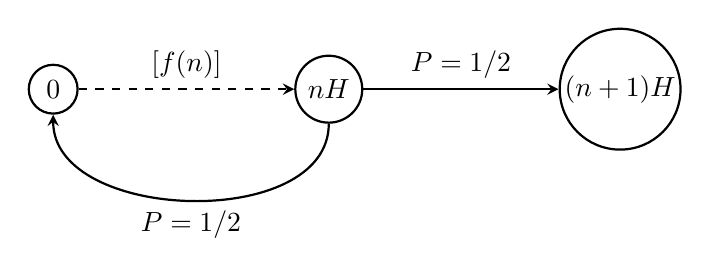
\begin{tikzpicture}[>=stealth,thick]
  \node[draw,circle,minimum size=0.62cm,inner sep=1pt] (zero) at (0,0) {$0$};
  \node[draw,circle,minimum size=0.85cm,inner sep=1pt] (nh) at (3.5,0) {$nH$};
  \node[draw,circle,minimum size=1.15cm,inner sep=1pt] (nph) at (7.2,0) {$(n+1)H$};
  \draw[->,dashed] (zero) -- node[above] {$\E[f(n)]$} (nh);
  \draw[->] (nh) -- node[above] {$P=1/2$} (nph);
  \draw[->] (nh.south) to[out=-90,in=-90] node[below] {$P=1/2$} (zero.south);
\end{tikzpicture}
\end{center}

The state before $(n+1)$ heads in a row (denoted as $(n+1)H$) must be $n$ heads in a
row (denoted as $nH$). It takes an expected $\E[f(n)]=2^{n+1}-2$ tosses to reach $nH$.
Conditioned on state $nH$, there is a $1/2$ probability it will go to $(n+1)H$ (the new
toss yields $H$) and the process stops. There is also a $1/2$ probability that it will go to the
